\chapter{Convolutional Neural Network}
\textbf{Convolutional Neural Network} (CNN) are particular types of neural network
feed forward. Their goal is to use multiple layers, stacked one on top of the other,
in order to extract input-related features. These layers are organized in a
hierarchical way, where the highest level calculates more global, more invariant
features.

Unlike the networks seen so far, CNNs organize weights using 3 dimensions. From
this point on, we will talk about the weights also considering the \textbf{volume}.
These volumes arise because the input consists of spatial dimensions (image width and
height) along with multiple input channels (e.g., RGB for color images). Each
neuron in a CNN acts as a filter, processing the entire spatial dimensions and
all input channels simultaneously. The output of each layer is another volume,
where the depth corresponds to the number of filters (or neurons) in the hidden
layer.

\begin{figure}[!ht]
    \centering
    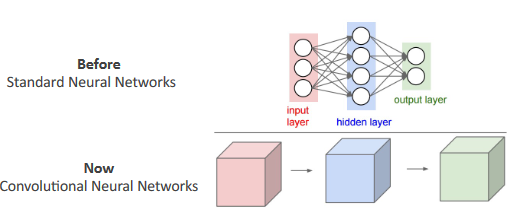
\includegraphics[width=0.5\textwidth]{img/CNN/weights.png}
    \caption{Weights representation in Feed Forward vs CNN.}
    \label{fig:weights}
\end{figure}

This particular type of network is widely used in the field of digital signal
processing, such as image or audio signals. If we look at image processing, this
kind of neural network offers a much more cost-effective approach than traditional
feed forward.

The most significant difference lies in how connections are structured. In a
feed forward network, each input neuron is fully connected to all neurons in the
next layer. This results in a significant complexity challenge. For instance,
with an image of $100 \times 100$ pixels, the input to the network is a vector
of $10,000$ pixels, leading to an enormous number of connections.

CNNs, on the other hand, introduce local connectivity, where each neuron focuses
on a small, localized portion of the image in each channel (\textbf{Local
    connectivity}). This drastically reduces the number of neurons and connections
required. For example, if the input image has dimensions $1000 \times 1000 \times 3$
(width, height, and 3 color channels), a single neuron could use a $5 \times 5 \times 3$
set of parameters. This is because the neuron processes a $5 \times 5$ spatial
region across all channels of the previous layer, a property referred to as full
depth connectivity.

\begin{figure}[!ht]
    \centering
    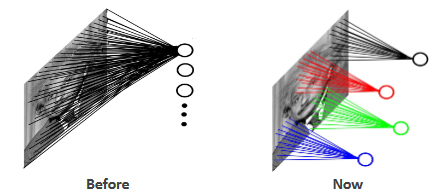
\includegraphics[width=0.5\linewidth]{img/CNN/localConn.png}
    \caption{Difference between the connections of neurons in a feed forward
        network and a CNN.}
    \label{fig:localConn}
\end{figure}

Also, another difference is that now, we have neurons organized in depth, we have
multiple neurons all looking the same region of the input volume, stacked along depth.

\begin{figure}[!ht]
    \centering
    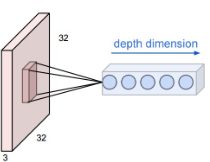
\includegraphics[width=0.25\linewidth]{img/CNN/depth.png}
    \caption{Organization of neurons in CNN}
    \label{fig:depth}
\end{figure}

In total we have $5\times 5\times 3$ weights to learn shared between each patch
of the image, this reduce a lot the number of learning parameter compared to
feed forward network. This concept is called \textbf{weights sharing}, which means
that the weights in the layer are shared across spatial positions.

In general, the structure of a CNN is organized so that it has a first part,
which includes convolutional layers, that extract the main characteristics from
the input. There is then a second part, composed of fully connected layer, which
performs the actual classification task. We can then represent this type of
network with a structure like the one shown in figure \ref{fig:cnnarc}.

\begin{figure}[!ht]
    \centering
    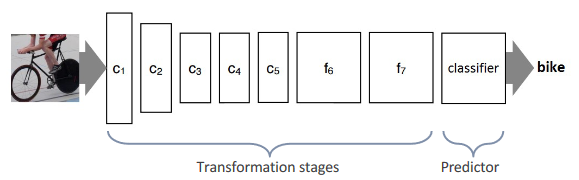
\includegraphics[width=\linewidth]{img/CNN/CNNarc.png}
    \caption{Overall CNN architecture.}
    \label{fig:cnnarc}
\end{figure}

The concept of \textbf{backpropagation} can still be utilized with this
architecture, which is a crucial aspect of training CNNs.

Respect to traditional neural networks, CNNs incorporate additional specialized
layers, such as \textbf{Spatial pooling} and \textbf{Local response normalization}.

These layers are useful to reduce computational complexity, increase invariance
and ease the optimization.
\section{CNNs components}
\subsection{Linear Convolution}
We begin by introducing the concept behind convolutional networks, namely the
concept of \textbf{linear convolution}. Convolution is a linear, local
(it applies on patches) and translation-invariant operator. To enrich the data
representation, we can use a \textbf{filter bank}, that is a collection of $Q$
sets of $K$ filters that allows to produce an output of $Q$ channel.

Let's see now, on a more mathematical level, what convolution represents. First we
introduce what we need:
\begin{itemize}
    \item $x = H \times W \times K$ is our input where $H$ represents the height
          dimension, $W$ the width dimension and $K$ the number of channels.
    \item $F = H' \times W' \times K \times Q$ is our filter bank where $Q$ is
          the number of filters that need to be apply to each channel.
    \item $y = (H - H' + 1) \times (W - W' + 1) \times Q$ is our output.
\end{itemize}

In addition to these, another very important thing to define is the \textbf{stride}.
The stride determines the step size for moving the filter across the input. By
default, the stride is set to 1, meaning the filter's center moves one pixel at
a time before being applied again.

\begin{note}
    A filter bank with 16 filters of depth $K$ produces an output with 16 channels.
\end{note}

The convolution is expressed by the following formula:
\begin{equation}
    y_{i, j, q} = y_q + \sum_{u = 0}^{H - 1}\sum_{v = 0}^{W - 1}\sum_{k = 1}^{K} x_{u + i, v + j, k} \cdot F_{u, v, k, q}
\end{equation}
where:
\begin{itemize}
    \item $y_q$ is the bias of the filter $F_q$;
    \item $x_{u + i, v + j, k}$ is the input patch of channel $k$;
    \item $F_{u, v, k, q}$ is the filter for the channel $k$ that computes output
          channel $q$.
\end{itemize}

\begin{figure}[!ht]
    \centering
    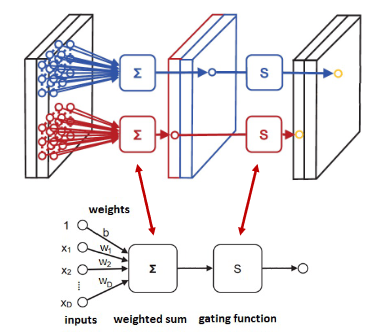
\includegraphics[width=0.25\linewidth]{img/CNN/Conv2Filter.png}
    \caption{Example of convolutional network with a filter bank of two elements.}
    \label{fig:conv2filter}
\end{figure}

We can apply filters in 2 way:
\begin{itemize}
    \item \textbf{Lattice structure}: a single filter is applied to a single
          channel ($K = 1$);
    \item \textbf{Multiple feature structure}: a single filter is applied to all
          channel of the input image $(K > 1)$.
\end{itemize}

In CNN, after the filter application we use a non linear activation function,
also called \textbf{gating function}: \textit{Sigmoid}, \textit{Tanh}, \textit{ReLU}
and \textit{SmoothReLU}.

\subsection{Spatial pooling}
We have already said that there are different types of layers in a CNN, one of
them is the \textbf{spatial pooling}.

The purpose of this layer is to subsample the image, reducing its spatial
dimensions and, in turn, the computational load. Additionally, spatial pooling
aggregates information from the image, enhancing translation invariance, which
makes the model more robust to variations in the exact spatial positions of
features. This is done in two main ways:
\begin{itemize}
    \item \textbf{avg pooling}: computing an average of the value of the pixels
          in the neighborhood:
          \begin{equation}
              y_{ijk} =\text{avg}_{p, q \in \Omega} x_{p, q, k}
          \end{equation}
    \item \textbf{max pooling}: taking the maximum value from the pixels in the
          neighborhood:
          \begin{equation}
              y_{ijk} = \max_{p, q \in \Omega_{i, j}} x_{p, q, k}
          \end{equation}
\end{itemize}

This is done channel by channel.
\subsection{Local Response Normalization}
\textbf{Local Response Normalization} layers have the objective of normalizing the
effect of contrast to improve the network invariance in this respect. This layer
also allows for improved optimization and sparsity (accuracy and speed).

In general, there are two ways of applying it:
\begin{itemize}
    \item \textbf{Within Channel}: operates independently on different feature
          channels, and also rescales each input feature basing on a local
          neighborhood.
          \begin{equation}
              y_{i, j, k} = x_{i, j, k} \left(k + \alpha \sum_{(u, v) \in \mathcal{N}(i, j)} x_{u, v, k}^2 \right)^{-\beta}
          \end{equation}
    \item \textbf{Across Channels}: operates independently at each spatial location
          and groups of channels. It also normalizes groups $G(k)$ of feature
          channels. Groups are usually defined in a sliding window manner.
          \begin{equation}
              y_{i, j, k} = x_{i, j, k} \left(k + \alpha \sum_{q \in G(k)} x_{i, j, q}^2 \right)^{-\beta}
          \end{equation}
\end{itemize}

\subsection{Input sensibility}
CNN are sensible to the input images, moreover we need a lot of data to train
from scratch a CNN. So we have to normalize images using:
\begin{itemize}
    \item \textbf{Local mean subtraction}
    \item \textbf{Normalization}
\end{itemize}
to have data centered in 0. To prevent overfitting we can use:
\begin{itemize}
    \item Weight decay;
    \item Dropout;
    \item Data augmentation: for example changing illuminants, flip the image,
          random crop and a geometric distortion.
\end{itemize}
Remember that is always better to accept new data.

\section{CNN Architectures}
Below, we will introduce some of the most famous CNN architectures. This is done
because the training from zero of one of these models requires a very large amount
of data and many computational resources.
\begin{itemize}
    \item \textbf{LeNet} is one of the first model that this is first create for
          the MNIST dataset. This network take in input a gray scale image of
          size $32 \times 32$.
          \begin{figure}[!ht]
              \centering
              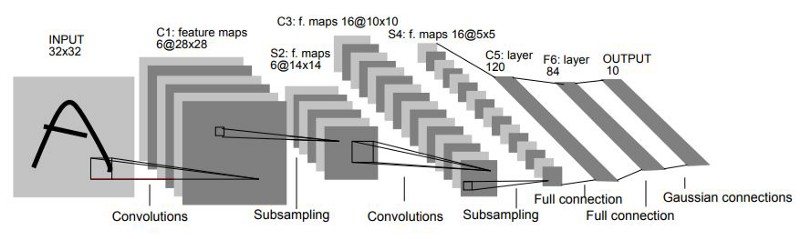
\includegraphics[width=0.45\linewidth]{img/CNN/LeNet-5.jpeg}
              \caption{LeNet}
              \label{fig:lenet}
          \end{figure}
    \item \textbf{AlexNet} was created for the ImageNet challenge and combines
          some convolutional layers with feed forward layers. It starts with a
          large convolutional level that is gradually reduced in order to encode
          the deeper layers of the more specific information in the task. In
          general we decrease filter dimension, increasing the depth channels.
          \begin{figure}[!ht]
              \centering
              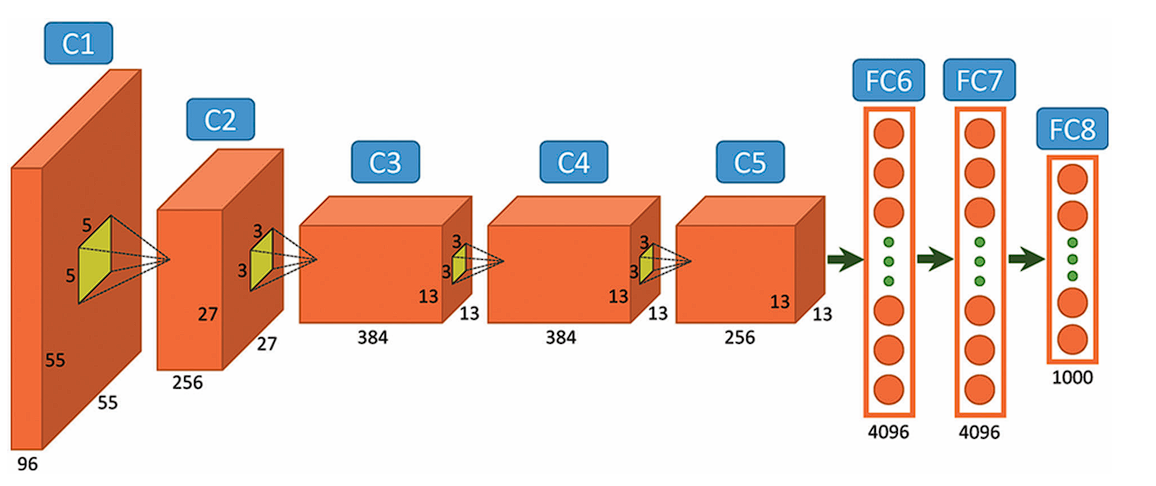
\includegraphics[width=0.45\linewidth]{img/CNN/alexNet.png}
              \caption{AlexNet}
              \label{fig:alexnet}
          \end{figure}
    \item \textbf{VGG} is a family of CNNs that consists of networks with varying
          numbers of convolutional layers. Compared to AlexNet, VGG uses smaller
          filters to reduce the number of parameters. Additionally, due to the
          concept of the \textbf{receptive field}, using smaller filters in multiple
          layers can achieve a similar receptive field to using a larger filter
          in a single layer. This allows VGG to maintain model depth while managing
          the number of parameters more efficiently.
          \begin{figure}[!ht]
              \centering
              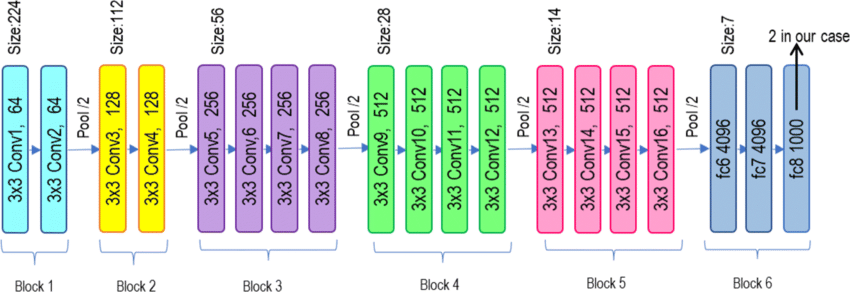
\includegraphics[width=0.45\linewidth]{img/CNN/VGG.png}
              \caption{VGG-19}
              \label{fig:vgg}
          \end{figure}
    \item \textbf{GoogLeNet} is one of the first networks to introduce the
          \textbf{module} concept. In particular, it uses the module called
          \textbf{inception} which is a part of the network, which can be stacked
          over other similar modules to get a larger network.

          As we are increasing the size of the network, we may encounter the
          problem of vanishing gradient. To solve this problem the creators introduce
          auxiliary output levels in different parts of the network in order to
          inject the gradient into different levels.

          This is done by creating a loss function which is a linear combination
          of the output, with an higher weights on final loss than the others losses.
          \begin{figure}[!ht]
              \centering
              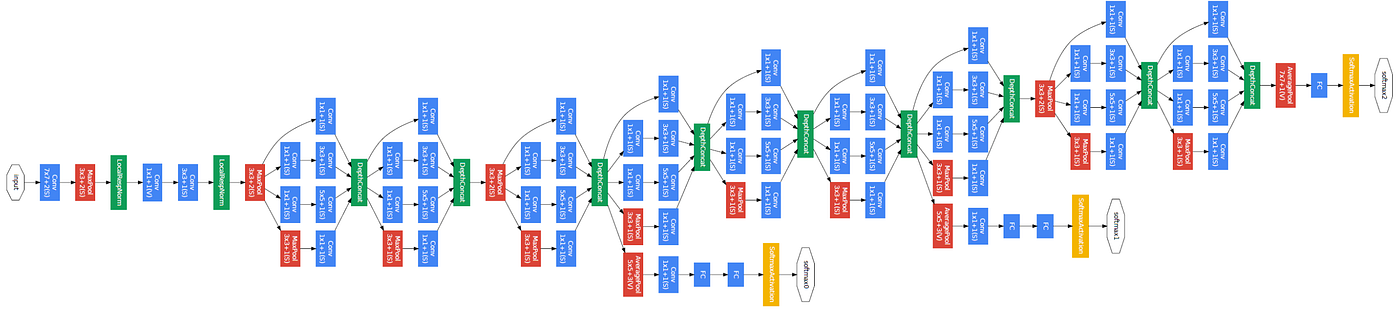
\includegraphics[width=0.45\linewidth]{img/CNN/GoogLeNet.png}
              \caption{GoogLeNet}
              \label{fig:GoogLeNet}
          \end{figure}
    \item \textbf{ResNet} is a network type that uses the idea of \textbf{residue}.
          The basic concept is to provide in input the identity function and let
          the network learn how to modify this function to approach the one you
          want to learn. The identity function is used because it can be easily
          implemented by adding the input to the result obtained at a particular
          point in the network. This is done to limit the vanishing gradient
          problem as the derivative of the identical function is always 1. With
          this trick you can implement much deeper networks.
          \begin{figure}[!ht]
              \centering
              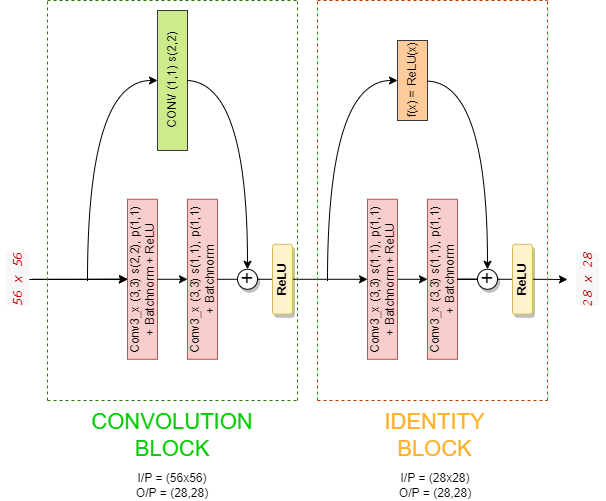
\includegraphics[width=0.25\linewidth]{img/CNN/ResNet.png}
              \caption{ResNet}
              \label{fig:resnet}
          \end{figure}
\end{itemize}

\begin{note}
    Usually we can use $1 \times 1$ convolution to squeeze information in depth
    channel without having impact on the spatial information.
\end{note}

\subsection{Transfert learning}
As mentioned above, it is not always possible to train a CNN from scratch. Depending on
the situation and the amount of data available. Generally we can train model from
scratch on a big dataset, then we can fine tune on our task dataset. In general,
one of the following techniques may be adopted:
\begin{itemize}
    \item New dataset is small and similar to original dataset: we can train a
          linear classifier on CNN features from higher layers;
    \item New dataset is large and similar to original dataset: we can Fine-tune
          the CNN;
    \item New dataset is small but very different from original dataset: we can
          train a linear classifier on CNN features from lower layers because we
          have to learn general features;
    \item New dataset is large and very different from original dataset: we can
          train CNN from scratch or fine-tune it
\end{itemize}

\section{Model Compression}
When developing a Deep Neural Network model, it is crucial to consider the devices
on which it will run, especially if the model is to be distributed to users. For
example, running a large language model (LLM) on a mobile device would not be
practical. Therefore, it's important to find the right balance between performance
and compatibility. One possible solution is to host the model in the cloud, but
this approach introduces challenges, such as network latency and privacy concerns.

An alternative approach is to create a more compact model that can run efficiently
on a mobile device while achieving performance similar to that of larger models.
An added advantage of this solution is that, due to its reduced size, the inference
process will be faster.

To achieve these results, several aspects were studied.
\subsection{Weight Sharing}
\textbf{Weight sharing} is a simple form of network reduction that involves
sharing weights between layers or structures within layers. Unlike other
compression techniques, weight sharing is typically applied before training the
original network, rather than compressing the model after training. This technique
reduces the network size and avoids sparsity. However, it is not always clear
how many and which weights should be shared before performance degradation becomes
unacceptable for a given network architecture and task.

An example of weight sharing can be seen in Convolutional layers, where each
neuron shares the same set of weights.

\subsection{Network pruning}
Pruning weights is one of the most commonly used techniques to reduce the number
of parameters in a pre-trained Deep Neural Network (DNN). This can lead to
reductions in storage and model runtime. Performance is usually maintained by
retraining the pruned network.

Iterative weight pruning prunes weights while retraining the network until the
desired trade-off between network size and accuracy is achieved. The simplest
pruning strategy involves setting a threshold to determine which weights or units
(in this case, the absolute sum of the magnitudes of incoming weights) are
removed. The threshold can vary for each layer or be global for the entire network.
Instead of setting a threshold, one can predefine a percentage of weights to be
pruned based on their magnitude, or a percentage aggregated by weights for each
layer. Typically, the weights with magnitudes closest to 0 are removed.

\textbf{Magnitude-based pruning (MBP)} is the most commonly used pruning technique
in DNNs due to its simplicity. It works well for a wide range of machine learning
models, including DNNs, across various tasks. In general, global MBP tends to
outperform layer-wise MBP because it provides more flexibility in determining
the amount of sparsity for each layer. This allows more important layers to remain
denser while less important layers contain more non-zero entries.

\subsubsection{Categorization of Pruning Techniques}
\begin{itemize}
    \item \textbf{Magnitude-based (iterative pruning + retraining)}: This technique
          removes the weights with the lowest absolute values based on a set
          threshold or percentage, either layer-wise or globally. The steps are
          as follows:
          \begin{enumerate}
              \item Choose a neural network architecture.
              \item Train the network until a reasonable solution is obtained.
              \item Prune the weights with magnitudes smaller than a threshold $\tau$.
              \item Retrain the network until a reasonable solution is obtained.
              \item Repeat step 3.
          \end{enumerate}
    \item \textbf{Methods that penalize the objective} with a regularization
          (L1, L2, etc.) term to force the model to learn a network with smaller
          weights and prune the smallest weights. This pruning technique is based
          on weight regularization, where we add a penalty term to the objective
          function to encourage the model's weights to approach zero. The smallest
          weights are then deleted. Typically, an L2 regularization is used, but
          care should be taken when using a more quadratic penalty as it can overly
          penalize larger weights.
    \item \textbf{Methods that compute the sensitivity of the loss function} when
          weights are removed, using this sensitivity as a criterion for removing
          weights that result in the smallest change in loss. \textbf{(Diagonal)
              Hessian-based pruning: Optimal Brain Damage}:
          \begin{enumerate}
              \item Choose a neural network architecture.
              \item Train the network until a reasonable solution is obtained.
              \item Compute the second derivatives for each parameter.
              \item Compute the saliencies for each parameter: $S_k = \frac{\delta^2E}{\delta^2 u_k} u_k^2$.
              \item Sort the parameters by saliency and delete low-saliency parameters.
              \item Repeat step 2.
          \end{enumerate}
    \item \textbf{Search-based approaches} that seek to learn or adapt a set of
          weights, links, or paths within the neural network, keeping those that
          are salient for the task.
\end{itemize}
\subsubsection{Structured vs. Unstructured Pruning}
Another important distinction to be made is between structured and unstructured
pruning techniques:
\begin{itemize}
    \item \textbf{Structured pruning} aims to preserve network density for
          computational efficiency (resulting in faster computation at the expense
          of less flexibility) by removing groups of weights.
    \item \textbf{Unstructured pruning} is unconstrained as to which weights or
          activations are removed, but the sparsity means that the dimensionality
          of the layers does not change.
\end{itemize}
Therefore, sparsity in unstructured pruning techniques generally provides good
performance at the expense of slower computation.

\textbf{Structured pruning via weight regularization}: Since standard pruning
leads to non-structured connectivity, structured pruning can be used to reduce
memory usage and increase speed. Hardware is more amenable to dealing with dense
matrix multiplications, especially when there are few non-zero entries in matrices
and tensors. Convolutional Neural Networks (CNNs) are particularly suitable for
this type of pruning since they consist of sparse connections.

\textbf{Group sparsity regularization}: Group sparse regularizers enforce a subset
of weight groupings (such as filters in CNNs) to be close to zero when trained
using stochastic gradient descent. For example, consider a convolutional kernel
represented as a tensor $K(i; j; s; :)$. The group-wise $L_1$-norm, $L_2$-norm
is given as:
\begin{equation*}
    \omega_{2, 1}(K) = \lambda \sum_{i, j, s} | \Gamma_{ijs} | = \lambda \sum_{i, j, s} \sqrt{\sum_{t= 1}^T K(i, j, s, t)^2}
\end{equation*}

Where $\Gamma_{ijs}$ is the group of kernel tensor entries $K(i; j; s; :)$, where
$(i;j)$ represents the pixel location in the $i$-th row and $j$-th column of the
image for the $s$-th input feature map. This regularization term forces certain
groups $\Gamma_{ijs}$ to be close to zero, which can be useful for pruning.

\subsection{Low rank matrix and tensor decomposition}
The idea starts from the observation that most weights are in the fully connected
layers, and that fully connected layers are implemented with a single matrix
multiplication.
\subsection{Knowledge distillation}
Involves learning a smaller network from a large network using supervision from
the larger network and minimizing the entropy, distance or divergence between
their probabilistic estimates. Probably the first work about KD is from Bucilua
et al. where they explored the idea of reducing model size by learning a student
network from an ensemble of models.
\begin{itemize}
    \item They use a teacher network to label a large amount of unlabeled data
          and train a student network using supervision from the pseudo labels
          provided by the teacher;
    \item They find performance is close to the original ensemble with $1000 \times$
          smaller network.
\end{itemize}

Hinton et al. showed a neural network knowledge distillation approach where a
small model is trained using supervision (class probability outputs) from the
original “teacher” model. They showed that learning from the larger network
outperformed the smaller network learning from scratch in the standard supervised
classification setup.
\subsection{Quantization}
\textbf{Quantization} is the process of representing values with a reduced number
of bits. In neural networks, this can be applied to weights, activations and
gradient values. Typically, when training on the GPU, values are stored in 32-bit
floating point (FP) single precision. Half-precision for floating point (FP-16)
and integer arithmetic (INT-16) are also commonly considered. INT-16 provides
higher precision but a lower dynamic range compared to FP-16. In FP-16, the result
of a multiplication is accumulated into a FP-32 followed by a down-conversion to
return to FP-16.

To speed up training, faster inference and reduce bandwidth memory requirements,
ongoing research has focused on training and performing inference with lower-precision
networks using integer precision (IP) as low as INT-8, INT-4, INT-2 or 1 bit
representations.

Designing such networks makes it easier to train such networks on CPUs, FPGAs,
ASICs and GPUs. Two important features of quantization are the range of values
that can be represented and the bit spacing.

For the range of signed integers with n bits, we represent a range of $[-2n-1, 2n-2]$
and for full precision (FP-32) the range is $\pm3.4e38$. For signed integers,
there are $2n$ values in that range and approximately $4.2e9$ for FP-32. FP can
represent a large array of distributions which is useful for neural network
computation, however this comes at larger computational costs when compared
to integer values.

For integers to be used to represent weight matrices and activations, a FP scale
factor is often used hence many quantization approaches involve a hybrid of mostly
integer formats with FP-32 scaling numbers. This approach is often referred to
as mixed-precision (MP). Different MP strategies have been used to avoid overflows
during training and/or inference of low resolution networks given the
limited range of integer formats.
\subsection{Low resource and efficient architectures}
\begin{figure}[!ht]
    \centering
    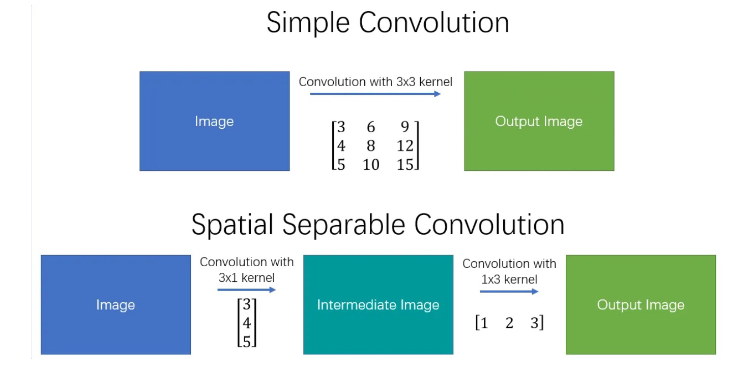
\includegraphics[width=0.5\linewidth]{img/CNN/spatialConv.png}
    \caption{Spatial Separable Convolution}
    \label{fig:spatialConv}
\end{figure}
\begin{itemize}
    \item \textbf{MobileNet}: is a sort of compression of CNN for embedded mobile
          vision application. They use depth-wise separable convolution (DSC) and
          2 hyperparameter that trade off latency and accuracy. DSC split the
          convolution in 2 steps, first filtering then combining outputs of each
          DSC filter, this is why it is referred as factorization approach.
    \item \textbf{SqueezeNet}: reduce the network architecture by reducing $3 \times 3$
          filters to $1\times1$ filters (squeeze layer). Reduce the number of
          input channels to $3 \times 3$ filters using squeeze layers and down
          sample later in the network to avoid the bottleneck of information
          through the network too early and in turn lead to better performance.
          A fire module is made up of the squeeze layer and an expand layer that
          is a mix of $1 \times 1$ and $3 \times 3$ convolution filters. The number
          of filters per fire module is increased as it gets closer to the
          last layer.
    \item \textbf{ShuffleNet}: uses point-wise group convolutions (i.e using a
          different set of convolution filter groups on the same input features,
          this allows for model parallelization) and channel shuffles (randomly
          shuffling helps information flow across feature channels) to reduce
          compute while maintaining accuracy. ShuffleNet is made up economical
          $3 \times 3$ depth-wise convolutional filters and replace $1 \times 1$
          layer with point-wise group convolutional followed by the channel
          shuffle. Unlike predecessor models, ShuffleNet is efficient for smaller
          networks.
    \item \textbf{DenseNet}: Gradients can vanish in very deep networks because
          the error becomes more difficult to backpropagate as the number of
          matrix multiplications increases. DenseNets address gradient vanishing
          connecting the feature maps of the previous layer to the inputs of the
          next layer, similar to ResNet skip connections. This reusing of features
          means the network efficient with its use of parameters. Although, deep
          and thin DenseNetworks can be parameter efficient, they do tradeoff
          with memory/speed efficiency in comparison to shallower yet wider network
          because all layer outputs need to be stored to perform backpropagation.
          However, DenseNets too can be made wider and shallower to become more
          memory efficient if required.
\end{itemize}